\documentclass[runningheads]{llncs}
\usepackage[T1]{fontenc}
\DeclareUnicodeCharacter{21D2}{\ensuremath{\Rightarrow}}
\DeclareUnicodeCharacter{00D7}{\ensuremath{\times}}
\DeclareUnicodeCharacter{03BB}{\ensuremath{\lambda}}
\usepackage{graphicx} % Required for inserting images
\usepackage{url}
\usepackage{amsmath}
\usepackage{amssymb}
\usepackage{booktabs}
\usepackage{array}
\usepackage{xcolor,xspace}
\usepackage{minted}
\usepackage[hidelinks]{hyperref}
\usepackage{newunicodechar}
\newunicodechar{⟷}{\ensuremath{\leftrightarrow}}

\newcommand{\ie}{\emph{i.e.,}\xspace}
\newcommand{\eg}{\emph{e.g.,}\xspace}
\newcommand{\ofs}{o\!f\!s}
\newcommand{\car}{\texttt{Cargo}\xspace}
\newcommand{\IR}{Isabelle2Rust\xspace}
\newcommand{\hol}{Isabelle/HOL\xspace}
\newcommand{\coq}{Rocq\xspace}
\newcommand{\thi}{Thingol\xspace}
\newcommand{\oml}{OCaml\xspace}
\newcommand{\TODO}[1]{{\textcolor{violet}{TODO: #1}}}
\newcommand{\yes}{\checkmark}
\newcommand{\partialyes}{$\triangle$}
\newcommand{\no}{$\times$}

\newcommand{\rprelude}{\textsc{Prelude}}

\setminted{
  fontsize=\scriptsize,
  breaklines=true,
  autogobble=true,
  frame=single,
  framesep=2mm,
  tabsize=2
}

% SETTA uses double-blind review.  Switch this flag to false for the
% camera-ready version.
\newif\ifanonymousreview
\anonymousreviewtrue

\begin{document}

\title{Rust2Isabelle: A Rust-to-Isabelle/HOL Backend for Aeneas}
\ifanonymousreview
\author{Anonymous Authors}
\institute{Anonymous Institution}
\else
\author{Zefeng Cheng \and Jun Liu \and Jiayi Lu \and Shenghao Yuan  \and Yongwang Zhao \and David Sanan}
%\authorrunning{F. Author et al.}
\institute{Zhejiang University, Hangzhou, China \and
\email{chengzf0898@gmail.com} \and
%\url{https://github.com/AeneasVerif/aeneas} \and
%\url{https://github.com/OpenSourceVerif/Aeneas2Isabelle}}
\fi
\date{August 2026}

\maketitle

\begin{abstract}
    Rust's ownership and borrowing discipline prevents broad classes of memory errors, but does not establish functional correctness.
Aeneas addresses this gap by translating a subset of safe Rust into pure functional models for several interactive theorem provers.
We present \texttt{Rust2Isabelle}, an Isabelle/HOL backend for Charon--Aeneas that translates Aeneas's typed functional intermediate representation, called the Pure AST into Isabelle theories.

The backend maps Pure constructs to corresponding Isabelle/HOL definitions while retaining Aeneas's functional representation of mutable borrows.
We also provide an Isabelle/HOL library, called the \rprelude{}, that defines the Rust primitives and library operations required by the generated theories.

We implement the backend in OCaml and evaluate it in two settings.
On the Aeneas regression suite, Isabelle accepts 23 generated theories that cover the main constructs of the supported Rust fragment.
In a complementary case study, \texttt{Rust2Isabelle} translates two components of Solana blockchain virtual machine into Isabelle/HOL theories.
Together, these results demonstrate the feasibility of automatically generating Isabelle/HOL models from supported safe Rust code and reveal gaps in the current library support.

    \keywords{Rust \and Isabelle/HOL \and Aeneas \and Formal Verification \and Functional Translation \and Code Generation}
\end{abstract}

\section{Introduction}
\label{sec:introduction}

Rust prevents broad classes of memory errors through its ownership and borrowing disciplines and has gained increasing adoption in systems software~\cite{jung2017rustbelt,li2024empirical}.
However, memory safety alone does not guarantee functional correctness or security~\cite{xu2021memory}. A memory-safe Rust program may still overflow, violate a protocol invariant, or produce an incorrect result~\cite{Edera}.
Formal verification provides a rigorous way to establish such functional-correctness properties by proving that a program satisfies a precise specification.

% Rust formal verification, Verus, Prusti Cresuot ... ATP,  for ITP, Charon-Aeneas LLBC benifits xxx supports xxx, currently not Isabelle/HOL.

% we select Rust2isabelle/HOL. Isabelle benifits xxx, 

% Cresuot-why3-Isabelle/HOL (why3 common experssion), Autocorrede (manually model in Isabelle/HOL). We select charon-Aeneas path xxx for the reason xxx.

Isabelle/HOL~\cite{nipkow2002isabelle} is a mature interactive theorem prover based on classical higher-order logic.
It supports recursive definitions, algebraic datatypes, reusable theorem libraries, and substantial proof automation~\cite{bohme2010sledgehammer,nelson2019scaling}.
In addition, it has supported several large-scale systems verification efforts~\cite{alkassar2008formal,becker2026nitro,zhao2019rely}, most notably the functional-correctness verification of the seL4 microkernel~\cite{sel4-sosp}.
These features make Isabelle/HOL a natural target for reasoning about the functional correctness of Rust programs.


However, manually constructing and maintaining a faithful Isabelle/HOL model of Rust programs requires considerable effort. 
% Such a model must account for Rust's rich type system. 
% A direct translation must handle ownership and borrowing without reintroducing unnecessary memory reasoning.
In particular, a direct translation need preserve Rust's ownership and borrowing discipline without reintroducing an explicit memory model.
The Charon--Aeneas~\cite{ho2025charon,ho2022aeneas} toolchain provides a reusable foundation for automating this process.
% We therefore build on the relatively mature Charon--Aeneas toolchain rather than developing the entire translation infrastructure 
% About the toolchain, 
Charon translates Rust compiler Mid-level Intermediate Representation (MIR) into the Low-Level Borrow Calculus (LLBC), a typed and structured intermediate representation designed for downstream program analysis.
Aeneas then consumes LLBC and uses symbolic execution to eliminate ownership and borrowing constructs, producing a Pure functional AST suitable for verification.
Aeneas currently provides extraction backends for F$^\star$~\cite{swamy2016dependent}, Rocq~\cite{bertot2013interactive}, HOL4~\cite{slind2008brief}, and Lean4~\cite{moura2021lean}, but it lacks support for Isabelle/HOL.

To fill this gap, we develop \texttt{Rust2Isabelle} as a new extraction backend for Aeneas.
It combines automatic generation of Isabelle/HOL theories with a companion library defining the Rust primitives used in the output.

We provide the following contributions.
\begin{itemize}
    \item \textbf{Rust2Isabelle Translation Rules}: We define translation rules from Rust to Isabelle/HOL. 
    These rules cover several Rust features, including types, expressions, mutable borrows, traits, const generics, and control flow.
    \item \textbf{Aeneas-Isabelle Prototype}: We implement a new Isabelle/HOL backend for Aeneas. 
    This backend generates complete Isabelle/HOL theory files from Rust code. 
    Our implementation is written in OCaml and integrates easily into the existing Aeneas ecosystem.
    \item \textbf{Evaluation}: We evaluate our approach and implementation using the official Aeneas test suite. 
    Additionally, we apply our tool to a key component of the real-world Solana~\cite{SolanaRBPF2} blockchain virtual machine as a case study.
\end{itemize}

% 1. Translation rules from Rust 2 Isabelle
% 2. compiler tool implementation + intergration
% 3. evaluation

{
\def\sectionautorefname{Section}
The rest of the paper is organized as follows.
\autoref{sec:background} reviews the relevant features of Rust, Aeneas's Pure AST, and Isabelle/HOL. 
\autoref{sec:design} presents the \texttt{Rust2Isabelle} workflow and the translation rules by language construct.
\autoref{sec:evaluation} combines construct-level coverage with an SBPF (Solana eBPF) virtual machine case study, Isabelle/HOL acceptance, and selected semantic properties.
Related work and the remaining limitations follow in~\autoref{sec:related} and~\autoref{sec:conclusion}.
}
\section{Background}
\label{sec:background}

This section reviews the source language, the functional representation produced by Aeneas, and the target logic used by \texttt{Rust2Isabelle}.

\subsection{Rust}

Rust is a systems programming language designed to provide memory safety
without garbage collection. Its type system assigns each value a unique
owner and controls access through borrowing.
A shared reference \texttt{\&T} permits read-only access and may be duplicated, whereas a mutable reference \texttt{\&mut T} permits exclusive access.
The borrow checker uses lifetimes to ensure that references do not outlive their owners and that mutable and shared access do not overlap in unsafe ways.
For safe Rust, these rules prevent errors such as use-after-free and unsynchronized data races without requiring a runtime memory manager~\cite{jung2017rustbelt}.

Rust programs also make extensive use of algebraic data types, pattern matching, traits, parametric polymorphism, and const generics.
These features are relevant to functional verification because they affect both the types of translated functions and the evidence passed to generic code.
Mutable borrows present the main semantic difficulty: an update through \texttt{\&mut T} must eventually be reflected in the value owned by the caller.
Rust's compiler represents checked programs using the MIR, a typed control-flow graph~\cite{rustc-mir} intended for compiler analyses and optimization rather than interactive proofs.

\subsection{Aeneas's Pure AST}

Aeneas takes as input LLBC, the typed and structured representation of Rust MIR produced by Charon~\cite{ho2025charon}. It symbolically executes LLBC using an ownership-centric semantics.
For its supported safe-Rust fragment, this process removes places, loans, and lifetime annotations and produces a side-effect-free functional representation called the Pure AST~\cite{ho2022aeneas}.
Shared borrows become ordinary values. A mutable borrow may produce a forward value together with a backward function.
After the borrowed value is updated, the backward function reconstructs the corresponding owner.
This representation captures the effect of mutation without carrying an explicit heap into the theorem prover.

The Pure AST also makes failures explicit. Operations that may panic or fail, such as checked arithmetic and bounds-checked indexing, return a result value.
Its declarations include types, functions, globals, trait declarations and implementations, const-generic parameters, and recursive groups.
Aeneas orders these declarations by dependency before passing them to a backend.
\texttt{Rust2Isabelle} starts at this boundary. It does not repeat Rust borrow checking or the symbolic execution from LLBC to Pure.

\subsection{Isabelle/HOL}

Isabelle is a generic interactive theorem prover that supports different
object logics.
Isabelle/HOL instantiates it with classical higher-order logic and is the logic used in this work~\cite{nipkow2002isabelle}.
An Isabelle theory contains named declarations and proofs and may import other theories.
Isabelle/HOL provides polymorphic types, datatypes, records, higher-order functions, and support for recursive and inductive definitions.
Its proof environment also offers automation tools such as Sledgehammer~\cite{bohme2010sledgehammer}.

Several properties of Isabelle/HOL affect the translation of the Pure AST.
Functions are total, and every HOL type is nonempty.
Declarations use commands such as \texttt{datatype}, \texttt{record}, \texttt{definition}, and \texttt{function}, and referenced types and constants must already be in scope.
These constraints shape the representation and translation choices presented in the next section.

\section{Translation to Isabelle/HOL}
\label{sec:design}

% predefined library with rust datatype modeled in Isabelle/HOL
This section presents the translation from Aeneas's Pure AST to Isabelle/HOL. We first describe the overall workflow and semantic support library, and then present the translation of types, expressions, mutable borrows, control flow, recursion, generics, and traits.

\subsection{Translation Overview}
\label{sec:workflow}

\autoref{fig:overview} presents the architecture of \texttt{Rust2Isabelle} within the Charon--Aeneas toolchain. Charon extracts LLBC from Rust, and Aeneas translates LLBC into a typed Pure AST together with the metadata required by subsequent extraction. These existing components are shown in grey. The Pure AST marks the boundary between Aeneas and the Isabelle backend.

% fix semantic support
\begin{figure}[!ht]
  \centering
  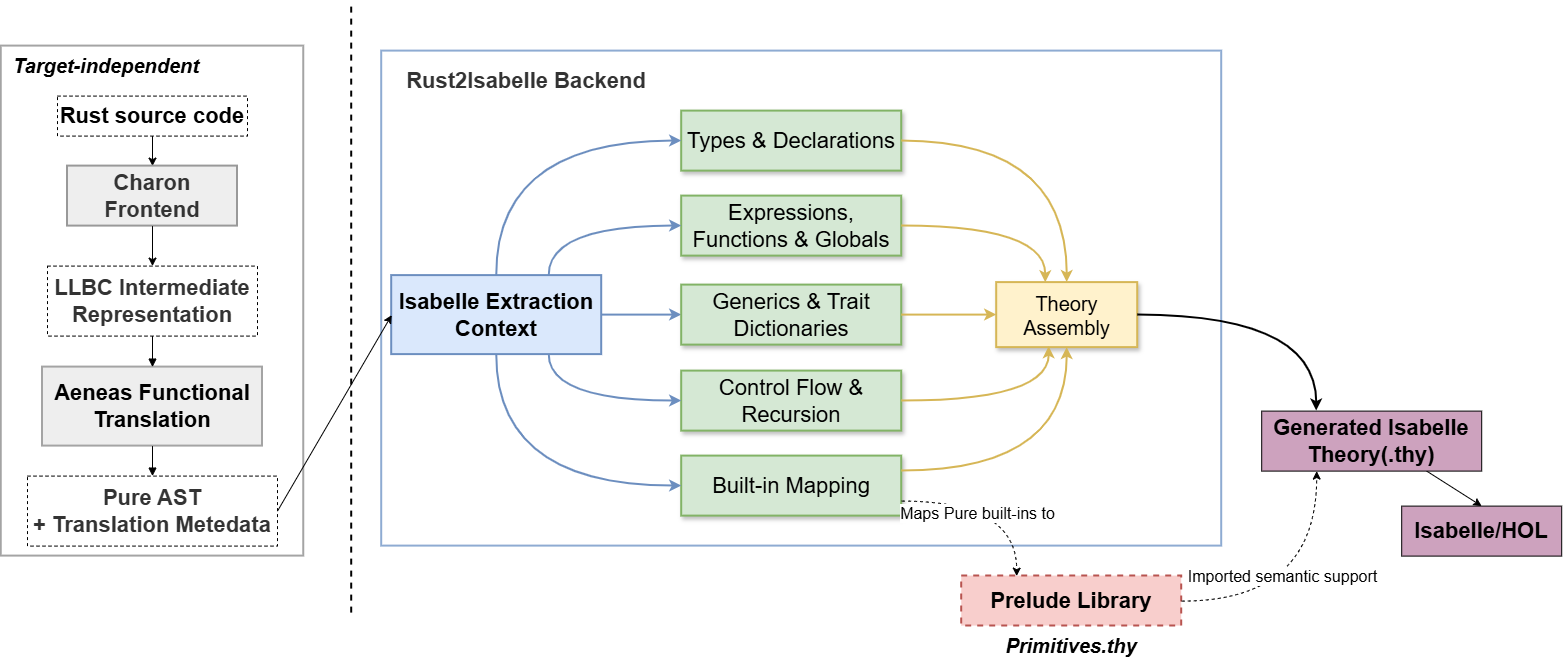
\includegraphics[width=\linewidth]{figure/structure.png}
  \caption{Architecture of \texttt{Rust2Isabelle} within the Charon--Aeneas toolchain. Highlighted components show the Isabelle-specific extensions, and the dashed connection indicates semantic support from the Prelude library.} 
  \label{fig:overview}
\end{figure}
\texttt{Rust2Isabelle} first constructs an Isabelle extraction context containing the Pure declarations, target names, built-in mappings, and dependency information.
Using this context, the backend translates each output module into an Isabelle theory.
% expressions
For each module, it then generates a \texttt{theory} header, imports the prelude library (denoted by \rprelude{}) and any user-specified theories, and places declarations in the dependency order supplied by Aeneas.

Pure constructs with direct Isabelle counterparts are translated into the corresponding types, terms, and declarations. For example, non-recursive functions and globals become typed \texttt{definition}s, whereas opaque declarations are introduced using \texttt{axiomatization}.
% rust specific feature make use of the predefined datatype and built-ins provided in the Prelude library
Operations without direct counterparts rely on the target-specific semantic support provided by the \rprelude{}, described in \autoref{sec:primitives}.

The current translation remains partial in several cases.
Termination obligations for singly recursive functions are admitted using Isabelle's \texttt{sorry}.
% no represented abstractly
% where we use axiomatization is 1.../2...
General loops and mutually recursive functions are currently represented abstractly, while unsupported built-ins may introduce \texttt{axiomatization} commands.
% Source-opaque
Source-opaque declarations are also abstract by design.
We distinguish these assumptions from fully defined translations in the evaluation.

\subsection{Rust Primitives in Isabelle/HOL}
\label{sec:primitives}

Following Aeneas's backend design, we implement the \rprelude{} as a fixed Isabelle/HOL theory that provides target-side semantics for the basic Rust primitives.
Recognized built-ins are mapped to definitions in the \rprelude{} or Isabelle/HOL. For example, Rust's \texttt{Option<T>} reuses Isabelle's \texttt{'a option} type and its \texttt{None} and \texttt{Some} constructors.

We next present the result monad, machine integers, and primitives for arrays, slices, and vectors.

% From the design principle of Aeneas, we define an Isabelle/HOL
% theory \texttt{Primitives.thy} to represent the basic Rust primitives.

% Generated theories rely on the \rprelude{} library for operations that have no
% direct Isabelle counterpart.  The library is implemented as the Isabelle
% theory \texttt{Primitives.thy}.  The backend identifies built-in types,
% constructors, functions, and trait instances by their Aeneas IDs.  Explicit
% lookup tables then map these IDs to Isabelle names. For example, Pure result constructors map to
% \texttt{Ok} and \texttt{Fail}, assertions map to \texttt{massert}, and array
% updates map to the corresponding prelude operation.  Ordinary Isabelle types
% such as \texttt{option} are reused where their constructors have the required
% shape.

\subsubsection{Result Type and Monadic Style} To represent fallible computations in the Pure AST, including panics, failed assertions, arithmetic overflow, and out-of-bounds indexing, the \rprelude{} library defines a corresponding result type: 

\begin{equation}
  \alpha\;\mathit{result}
  \triangleq \mathit{Ok}\;\alpha
  \mid \mathit{Fail}\;\mathit{error}
  \label{eq:result}
\end{equation}
The \texttt{error} type follows the Pure AST and contains two constructors: \texttt{Failure} represents panics, failed assertions, and other runtime errors, while \texttt{OutOfFuel} is retained for fuel-bounded computations.

Computations over \texttt{result} use the usual \texttt{return} and
\texttt{bind} operations.  The former wraps a value in \texttt{Ok}, while the latter passes a successful value to the continuation and propagates \texttt{Fail}.
\begin{equation}
  \mathit{bind}\;r\;f
  \triangleq
  \begin{cases}
    f\;x & \text{if } r = \mathit{Ok}\;x,\\
    \mathit{Fail}\;e & \text{if } r = \mathit{Fail}\;e.
  \end{cases}
  \label{eq:result-bind}
\end{equation}
% \begin{equation}
%   \mathit{bind}\;r\;f
%   \triangleq
%   \mathsf{case}\ r\ \mathsf{of}\
%     \mathit{Ok}\;x \Rightarrow f\;x
%     \mid
%     \mathit{Fail}\;e \Rightarrow \mathit{Fail}\;e.
%   \label{eq:result-bind}
% \end{equation}
For readability, the \rprelude{} provides a do-bind notation:
\begin{equation}
  \mathtt{x}\leftarrow\mathtt{m};\ \mathtt{e}
  \quad\triangleq\quad
  \mathit{bind}\;m\;(\lambda x.\,e)
  \label{eq:do-bind}
\end{equation}
Here, \(\equiv\) denotes syntactic equivalence rather than logical equivalence.
For example, \autoref{fig:do-bind-translation} shows how two sequential
arithmetic operations are translated using the result monad.

\begin{figure}[!ht]
\centering
\begin{minipage}[t]{0.45\textwidth}
\centering
\begin{minted}[
  frame=none,
  linenos,
  numbersep=4pt,
  xleftmargin=1.5em,
  fontsize=\small
]{rust}
// The Rust source
fn add_then_mul(
    a: u32,
    b: u32,
    c: u32,
) -> u32 {
    let x = a + b;
    x * c
}
\end{minted}
\end{minipage}
\hfill
\vrule{}
\hfill
\begin{minipage}[t]{0.5\textwidth}
\centering
\begin{minted}[
  frame=none,
  linenos,
  numbersep=4pt,
  xleftmargin=1.5em,
  fontsize=\small
]{isabelle}
(* The generated Isabelle/HOL *)
definition add_then_mul
  :: "u32 ⇒ u32 ⇒ u32
      ⇒ u32 result"
where
  "add_then_mul a b c =
    (x <- u32_add a b;
     u32_mul x c)"
\end{minted}
\end{minipage}
\caption{Translation of sequential Rust arithmetic using the result monad.}
\label{fig:do-bind-translation}
\end{figure}
The binding passes the result of \texttt{u32\_add} to \texttt{u32\_mul} when the addition succeeds. If the addition fails, the same failure is returned without evaluating the multiplication.

Assertions use the same mechanism.  The operation \texttt{massert} returns \(\mathit{Ok}\;()\) when its condition holds and \(\mathit{Fail}\;\mathit{Failure}\) otherwise. It can therefore be composed with other fallible computations through \texttt{bind}.

\subsubsection{Machine Integers}

Although Isabelle/HOL provides fixed-width word types, the \rprelude{} represents each Rust integer type $\tau$ using the unbounded type \texttt{int}, following Aeneas's backend-independent scalar interface.
Bounded and wrapping operations are defined using explicit range checks and modular reduction. Each value $x$ of type $\tau$ must satisfy a
well-formedness predicate:
\begin{equation}
  \mathit{wf}_\tau(x) \triangleq
  \min(\tau) \leq x \land x \leq \max(\tau)
\end{equation}

For an unsigned $b$-bit type $u_b$ and a signed $b$-bit type $i_b$, the valid ranges are $[0, 2^b-1]$ and $[-2^{b-1}, 2^{b-1}-1]$, respectively.
The present model fixes \texttt{usize} and \texttt{isize} to 64 bits.

A failure-producing scalar operation returns $\mathit{Fail}(\mathit{Failure})$ when its mathematical result lies outside the range of $\tau$. For example, scalar addition is defined as follows:
\begin{equation}
    \mathit{scalar\_add}_\tau(x,y) \triangleq
    \begin{cases}
        \mathit{Ok}(x+y) & \text{if }\mathit{wf}_\tau(x+y),\\
        \mathit{Fail}(\mathit{Failure}) & \text{otherwise.}
    \end{cases}
\end{equation}

For a $b$-bit integer type $\tau$, wrapping operation maps any mathematical integer $x$ into valid range of $\tau$.
It first computes $x$ modulo $2^b$. Then, for a signed type, values greater than or equal to $2^{b-1}$ are converted to negative values.
Otherwise, it returns the modulo value.
\begin{equation}
  \mathit{scalar\_wrap}_\tau(x) \triangleq
  \begin{cases}
    (x \bmod 2^{b}) - 2^b
      & \text{if }\tau\text{ is signed type}
        \land x \bmod 2^{b} \geq 2^{b-1},\\
    x \bmod 2^{b} & \text{otherwise.}
  \end{cases}
\end{equation}

The \rprelude{} library also defines overflow-checking operations, which return a tuple of wrapping operation result and a boolean overflow flag.
Floating-point scalars are not yet supported in the current scalar model.
% In contrast, checked operations (\eg $\mathit{add\_nooverflow}$) may fail. 
% They succeed only when the result remains within the valid bound; otherwise, they return failure information. 
% We formalize this behavior for the `addition with no overflow' operation as follows:
% \begin{equation}
%   \mathit{add\_nooverflow}_\tau(x,y) \triangleq
%   \begin{cases}
%     \mathit{Ok}(x+y) & \text{if }\mathit{wf}_\tau(x+y),\\
%     \mathit{Fail}(\mathit{Failure}) & \text{otherwise.}
%   \end{cases}
%   \label{eq:checked-add}
% \end{equation}

% Wrapping operations reduce modulo $2^{w_\tau}$ and reinterpret the result as a
% signed value when required.  Division and remainder use an explicit
% truncation-toward-zero definition because Isabelle integer division differs
% from Rust for negative operands.  Casts, shifts, bit operations, checked
% operations, and overflowing operations are defined from the same range and
% width information.  The present model fixes \texttt{usize} and
% \texttt{isize} to 64 bits.

% Type synonyms keep the resulting proof terms small, but do not prevent a user
% from applying a generated function to an out-of-range integer.  Theorems about
% public functions must therefore assume $\mathit{wf}_\tau$ for scalar inputs.
\subsubsection{Arrays, Slices, and Vectors}

Aeneas treats selected array, slice, and \texttt{Vec} operations from Rust's \texttt{core} and \texttt{alloc} libraries as built-ins. Rather than translating their library implementations, the backend maps them to executable definitions in the \rprelude{}.
These definitions support construction, length, indexing, update, range slicing, and mutable access.  Mutable access is discussed further in \autoref{sec:mutable-borrows}.

Arrays, slices, and vectors are represented by Isabelle/HOL lists, abstracting away their different memory layouts.
Consequently, neither the length parameter of \texttt{[T; N]} nor the capacity of \texttt{Vec<T>} is encoded in the target type.
The predicate \texttt{array\_wf} relates the erased parameter \texttt{N} to the length of the representing list.

Indexing performs an explicit bounds check and returns \texttt{Fail Failure} when the index is invalid.  Mutable indexing additionally returns a function for updating the original list:
\begin{equation}
  \mathit{index\_mut}(a,i) \triangleq
  \begin{cases}
    \mathit{Ok}\bigl(a[i],\lambda v.\,a[i:=v]\bigr)
      & \text{if }0\leq i<|a|,\\
    \mathit{Fail}\;\mathit{Failure}
      & \text{otherwise.}
  \end{cases}
  \label{eq:index-update}
\end{equation}
Here, \(|a|\) is the length of \(a\), and \(a[i:=v]\) replaces its \(i\)-th element with \(v\).  The returned function is the backward function used to reconstruct the list after mutation.

The \rprelude{} also provides the trait implementations required for
collection indexing and vector-to-slice dereferencing. Unsupported unchecked indexing returns \texttt{Fail Failure}.

\subsection{Types and Type Declarations}
\label{sec:types}

The backend translates both type expressions and type declarations. The principal translation rules are summarized in~\autoref{tab:type-map}.

\begin{table}[!ht]
  \centering
  \caption{Translation of Pure types and type declarations.}
  \label{tab:type-map}
  \begin{tabular}{@{}p{0.39\textwidth}p{0.54\textwidth}@{}}
    \toprule
    \textbf{Pure/Rust construct} & \textbf{Isabelle representation} \\
    \midrule
    \multicolumn{2}{@{}l}{\emph{Type expressions}}\\
    Boolean, character, unit
      & \texttt{bool}, \texttt{char}, \texttt{unit} \\
    Rust machine integers
      & Integer types using \texttt{int} based on \rprelude{} \\
    Tuple $(T_1,\ldots,T_k)$
      & Product type using \texttt{$\times$} \\
    Function $T_1\to T_2$
      & Function type using \texttt{$\Rightarrow$} \\
    Array, slice, and vector
      & List type using \texttt{'a list} based on \rprelude{} \\
    \midrule
    \multicolumn{2}{@{}l}{\emph{Type declarations}}\\
    Rust enum
      & \texttt{datatype} \\
    Non-recursive named struct
      & \texttt{record} \\
    Recursive struct
      & \texttt{datatype} \\
    Tuple struct / empty struct
      & Product type / \texttt{unit} \\
    Opaque type / empty enum
      & \texttt{typedecl} \\
    \bottomrule
  \end{tabular}
\end{table}
Boolean, character, unit, tuple, and function types map directly to their corresponding HOL types.
Rust type parameters such as \texttt{T} are translated to Isabelle type variables such as \texttt{'a}, making the generated functions polymorphic.
\autoref{fig:type-declaration-example} illustrates the translation of three representative Rust type declarations.

\begin{figure}[!ht]
\centering
\begin{minipage}{0.88\linewidth}
\begin{minipage}[t]{0.36\textwidth}
\begin{minted}[
  frame=none,
  linenos,
  numbersep=4pt,
  fontsize=\small
]{rust}
enum Flag {
  Off,
  On,
}

struct Point {
  x: u32,
  y: u32,
}

struct Node {
  next: Option<Box<Node>>,
}

struct Pair(u32, bool);
\end{minted}
\end{minipage}
\hfill
\vrule{}
\hfill
\begin{minipage}[t]{0.44\textwidth}
\begin{minted}[
  frame=none,
  linenos,
  numbersep=4pt,
  fontsize=\small
]{isabelle}
datatype Flag_t =
    Flag_Off
  | Flag_On

record Point_t =
  Point_x :: "u32"
  Point_y :: "u32"

datatype Node_t =
  mkNode_t
    (Node_next :
      "Node_t option")

type_synonym Pair_t =
  "u32 × bool"
\end{minted}
\end{minipage}
\end{minipage}
\caption{Translation of representative Rust type declarations.}
\label{fig:type-declaration-example}
\end{figure}
Each variant of the Rust enum becomes a constructor of the Isabelle datatype.
The recursive \texttt{Node} declaration is also translated into a datatype, since Isabelle records cannot be recursive. Its named constructor arguments retain the source field names.
In contrast, the non-recursive \texttt{Point} declaration becomes a record, and its \texttt{x, y} fields are represented by record selectors.

Tuple structs are represented by product types, while empty structs use
\texttt{unit}.  Opaque types and empty enums are represented by
\texttt{typedecl}.  The latter is an over-approximation because every
Isabelle/HOL type is nonempty.

\subsection{Expression Translation}
\label{sec:expressions}

Typed Pure expressions are translated recursively into Isabelle terms.
The translation follows the structure of the Pure AST and maps each expression form to its corresponding Isabelle syntax.~\autoref{tab:expression-map} summarizes the main translation rules.

\begin{table}[!ht]
  \centering
  \caption{Translation of common Pure expressions.}
  \label{tab:expression-map}
  \small
  \begin{tabular}{@{}p{0.42\textwidth}p{0.56\textwidth}@{}}
    \toprule
    \textbf{Pure expression} & \textbf{Isabelle term} \\
    \midrule
    Variable or literal
      & \texttt{x} or \texttt{c} \\
    Function application
      & \texttt{f e$_1$ $\ldots$ e$_n$} \\
    Lambda
      & \texttt{$\lambda$x. e} \\
    Conditional
      & \texttt{if e$_0$ then e$_1$ else e$_2$} \\
    Pattern match
      & $\mathtt{case}\ e_0\ \mathtt{of}\ 
     p_1 \Rightarrow e_1 \mid \cdots \mid p_n \Rightarrow e_n$ \\
    Non-monadic binding
      & \texttt{let x = e$_1$ in e$_2$} \\
    Monadic binding
      & \texttt{x $\leftarrow$ e$_1$; e$_2$} \\
    Tuple or ADT construction
      & \texttt{(e$_1$, \ldots, e$_n$)} or
        \texttt{C e$_1$ $\ldots$ e$_n$} \\
    Record projection
      & \texttt{field r} \\
    Record update
      & \texttt{r(\textbar{} field := e \textbar{})} \\
    \bottomrule
  \end{tabular}
\end{table}

Most expression forms are translated structurally, with function and constructor arguments retaining their order in the Pure AST. Field access is a target-specific exception. Since Isabelle record selectors are functions, an access \texttt{r.f} is translated into \texttt{f r}. Record updates use Isabelle's form \texttt{r(\textbar{} f := e \textbar{})}. Parentheses are added when necessary to preserve the grouping of nested expressions.

Pure let-expressions are translated either as ordinary Isabelle
\texttt{let}-bindings or, when marked as monadic in the Pure AST, using the do-bind notation described in \autoref{sec:primitives}.

\subsection{Mutable Borrows}
\label{sec:mutable-borrows}
Mutable borrows require additional functional structure.  A mutable reference
allows a callee to read a value and later propagate its updated value back to
the owner.  Since the Pure AST contains neither mutable memory locations nor a
heap, returning only the borrowed value would lose the information needed to
update its owner.  Aeneas therefore represents a mutable borrow using a
forward value and a backward function~\cite{ho2022aeneas}.  The forward value
provides the current contents of the borrow.  When the borrow ends, the
backward function receives its final value and reconstructs the updated
owners.

The function in \autoref{backward translation} demonstrates why the backward function is necessary. Depending on \texttt{b}, the returned mutable reference refers either to \texttt{x} or to \texttt{y}.  The backward function records this choice so that a later update can be propagated to the correct argument.

To avoid name collisions, the backend appends a trailing prime to Rust identifiers that conflict with Isabelle keywords or predefined constants.
For example, in \autoref{backward translation}, the Rust function \texttt{choose} is renamed to \texttt{choose'}.

\begin{figure}[H]
\centering
\begin{minipage}[t]{0.4\textwidth}
\centering
\begin{minted}[frame=none, linenos, numbersep=4pt, xleftmargin=1.5em, fontsize=\small]{rust}
fn choose<'a, T>(
    b: bool,
    x: &'a mut T,
    y: &'a mut T,
) -> &'a mut T {
    if b { x } else { y }
}
\end{minted}
\end{minipage}
\hfill
\vrule{}
\hfill
\begin{minipage}[t]{0.5\textwidth}
\centering
\begin{minted}[frame=none, linenos, numbersep=4pt, fontsize=\small]
{isabelle}
definition choose'
  :: "bool ⇒ 't ⇒ 't ⇒ 
     ('t × ('t ⇒ 't × 't)) result"
where
  "choose' b x y =
    (if b then
       let back = λx'. (x', y)
       in Ok (x, back)
     else
       let back = λy'. (x, y')
       in Ok (y, back))"
\end{minted}
\end{minipage}
\caption{Translation of a mutable borrow into a value and a backward function.}
\label{backward translation}
\end{figure}

The first component of the returned pair is the selected value, and the second is its backward function.  When \texttt{b} is true, updating the borrowed value to \(x'\) and applying the backward function produces \((x',y)\).  When \texttt{b} is false, an updated value \(y'\) produces \((x,y')\).
The update therefore reaches exactly the selected owner.  The Isabelle backend preserves this functional representation directly, without introducing a target heap or a separate alias relation.

\subsection{Control flow and Recursion}
\label{sec:recursion}

Conditionals and pattern matching translate directly into Isabelle \texttt{if} and \texttt{case} expressions, as shown in \autoref{tab:expression-map}.
Loops and recursive functions require separate treatment because Isabelle/HOL requires recursive definitions to be terminating.
Termination is undecidable in general, but Isabelle can prove it for many common cases when supplied with a variant, namely a value in a well-founded order that strictly decreases on every recursive call or continuing loop iteration.
The current backend does not obtain such variants from the Rust source or generate the corresponding decreasingness proofs.

A translated loop consists of a body function describing one iteration and the abstract \texttt{loop} operator provided by the \rprelude{}.
The body either propagates a failure, continues with a new state, or terminates with a break value:

\begin{equation}
\begin{aligned}
 \mathit{control\_flow}(S,B)
   &\triangleq \mathit{LoopContinue}\;S
      \mid \mathit{LoopBreak}\;B\\
 \mathit{loop}\ f\ s
   &\triangleq \mathsf{case}\ f\ s\ \mathsf{of}\\
   &\quad \mathit{Fail}\ e
      \Rightarrow \mathit{Fail}\ e \quad\mid \\
   &\quad \mathit{Ok}(\mathit{LoopBreak}\ b)
      \Rightarrow \mathit{Ok}\ b \quad\mid \\
   &\quad\mathit{Ok}(\mathit{LoopContinue}\ s')
      \Rightarrow \mathit{loop}\ f\ s'.
\end{aligned}
\label{eq:loop}
\end{equation}

The \texttt{loop} operator is axiomatized by the unfolding equation in \autoref{eq:loop}.
Repeated unfolding determines the result of an execution that eventually reaches \texttt{Fail} or \texttt{LoopBreak}.
Executions that continue indefinitely remain unspecified, so this encoding does not establish termination of the source loop.

A variant-based proof applies only to terminating programs.
Preserving genuinely divergent executions would instead require an explicit divergence-aware representation, as provided by the HOL4 backend.
The current Isabelle loop operator leaves such executions unspecified.

\begin{figure}[!ht]
\centering
\begin{minipage}{0.88\linewidth}
\begin{minipage}[t]{0.36\linewidth}
\vspace{0pt}
%\centering
\begin{minted}[
  frame=none,
  linenos,
  numbersep=4pt,
  fontsize=\small
]{rust}
while i < max {
  i += 1;
}
  i
\end{minted}
\end{minipage}
\hfill
\vrule{}
\hfill
\begin{minipage}[t]{0.56\linewidth}
\vspace{0pt}
%\centering
\begin{minted}[
  frame=none,
  linenos,
  numbersep=4pt,
  fontsize=\small
]{isabelle}
if i < max' then
  (i1 <- u32_add i (1 :: u32);
   Ok (LoopContinue i1))
else
  Ok (LoopBreak i)
\end{minted}
\end{minipage}
\end{minipage}
\caption{Translation of a Rust loop into a single-step loop body.}
\label{fig:loop-translation}
\end{figure}

% \begin{figure}[!ht]
% \centering
% \begin{minipage}[t]{0.34\textwidth}
% \begin{minted}[
%   frame=none,
%   linenos,
%   numbersep=4pt,
%   fontsize=\small
% ]{rust}
% fn iter(max: u32) -> u32 {
%     let mut i = 0;
%     while i < max {
%         i += 1;
%     }
%     i
% }
% \end{minted}
% \end{minipage}
% \hfill
% \vrule{}
% \hfill
% \begin{minipage}[t]{0.59\textwidth}
% \begin{minted}[
%   frame=none,
%   linenos,
%   numbersep=4pt,
%   fontsize=\small
% ]{isabelle}
% definition iter_loop_body
%   :: "u32 ⇒ u32 ⇒
%       ((u32, u32) control_flow) result"
% where
%   "iter_loop_body max' i =
%     (if i < max' then
%        (i1 <- u32_add i (1 :: u32);
%         Ok (LoopContinue i1))
%      else
%        Ok (LoopBreak i))"

% definition iter_loop
%   :: "u32 ⇒ u32 ⇒ u32 result"
% where
%   "iter_loop max' i =
%      loop (λi1. iter_loop_body max' i1) i"

% definition iter :: "u32 ⇒ u32 result"
% where
%   "iter max' = iter_loop max' (0 :: u32)"
% \end{minted}
% \end{minipage}
% \caption{Translation of a Rust loop using the \rprelude{} loop interface.}
% \label{fig:loop-translation}
% \end{figure}
In \autoref{fig:loop-translation}, the current value of \texttt{i} is the loop state. The generated body either continues with the incremented value or breaks with the final value. The backend additionally generates a wrapper that applies \texttt{loop} to this body and an entry definition that supplies the initial state.

Non-recursive functions use Isabelle's \texttt{definition} command.
Singly recursive functions use \texttt{function}, which generates a termination obligation requiring every recursive call to decrease according to a well-founded relation.
Mutually recursive groups are currently represented by typed \texttt{axiomatization}s because the backend does not yet generate joint recursive definitions.

\subsection{Generics and Traits}
\label{sec:traits}

Rust type parameters become polymorphic Isabelle type variables and require no runtime representation.
Const generics require a different treatment because Isabelle/HOL types cannot take const generics as type parameters.
We therefore translate a const-generic Rust structure into an Isabelle record, retaining \texttt{N} as a ghost field of type \texttt{usize}, while occurrences of \texttt{N} in function signatures become explicit \texttt{usize} parameters. \autoref{fig:const-generic-translation} illustrates this translation.

\begin{figure}[!ht]
\centering
\begin{minipage}{0.96\linewidth}
\begin{minipage}[t]{0.43\linewidth}
\vspace{0pt}
\centering
\begin{minted}[
  frame=none,
  linenos,
  numbersep=4pt,
  fontsize=\small
]{rust}
struct Buffer<const N: usize>{
    data: [u8; N],
}

fn wrap<const N: usize>(
    data: [u8; N],
) -> Buffer<N> {
    Buffer { data }
}
\end{minted}
\end{minipage}
\hfill
\vrule{}
\hfill
\begin{minipage}[t]{0.48\linewidth}
\vspace{0pt}
\centering
\begin{minted}[
  frame=none,
  linenos,
  numbersep=4pt,
  fontsize=\small
]{isabelle}
record Buffer_t =
  Buffer_N :: "usize"
  Buffer_data :: "u8 array"

definition wrap
  :: "usize ⇒ u8 array ⇒
      Buffer_t result"
where
  "wrap n data =
     Ok (| Buffer_N = n,
           Buffer_data = data |)"
\end{minted}
\end{minipage}
\end{minipage}
\caption{Translation of a const generic into a ghost field and an explicit
function parameter.}
\label{fig:const-generic-translation}
\end{figure}

Since \texttt{N} is a compile-time parameter in Rust, the ghost field exists only in the logical representation and does not correspond to runtime storage in the source program.
However, recording \texttt{n} alone does not guarantee that \texttt{Buffer\_data} contains exactly \texttt{n} elements.
The backend therefore generates the following well-formedness predicate:
\begin{equation}
  \mathit{Buffer\_wf}\;n\;v
  \;\triangleq\;
  \mathit{Buffer\_N}\;v = n
  \;\land\;
  \mathit{array\_wf}\;n\;(\mathit{Buffer\_data}\;v).
  \label{eq:buffer-wf}
\end{equation}

The predicate states that a translated buffer is well formed with respect to \texttt{n} when its ghost field equals \texttt{n} and its underlying list contains exactly \texttt{n} elements.

\begin{equation}
  \mathit{array\_wf}\;n\;\mathit{data}
  \;\Longrightarrow\;
  \mathit{result\_wf}\;
    (\mathit{Buffer\_wf}\;n)\;
    (\mathit{wrap}\;n\;\mathit{data}).
  \label{eq:wrap-wf}
\end{equation}

Equation~\eqref{eq:wrap-wf} is the preservation lemma for \texttt{wrap}. 
It states that if the input list represents an array of length \texttt{n}, then every successful result of \texttt{wrap} is a buffer whose ghost field is \texttt{n} and whose data field also has length \texttt{n}.
\texttt{Rust2Isabelle} automatically generates and proves this lemma to ensure that \texttt{wrap} preserves the const-generic constraint.
% \begin{figure}[!ht]
% \centering
% \begin{minipage}[t]{0.35\textwidth}
% \begin{minted}[
%   frame=none,
%   linenos,
%   numbersep=4pt,
%   fontsize=\small
% ]{rust}
% struct Buffer<const N: usize> {
%     data: [u8; N],
% }

% fn wrap<const N: usize>(
%     data: [u8; N],
% ) -> Buffer<N> {
%     Buffer { data }
% }
% \end{minted}
% \end{minipage}
% \hfill
% \vrule{}
% \hfill
% \begin{minipage}[t]{0.57\textwidth}
% \begin{minted}[
%   frame=none,
%   linenos,
%   numbersep=4pt,
%   fontsize=\small,
%   escapeinside=@@
% ]{isabelle}
% record Buffer_t =
%   Buffer_data :: "u8 array"

% definition Buffer_t_const_generic_wf
%   :: "usize ⇒ Buffer_t ⇒ bool"
% where
%   "Buffer_t_const_generic_wf n v ⟷
%      array_wf n (Buffer_data v)"

% definition wrap
%   :: "usize ⇒ u8 array ⇒ Buffer_t result"
% where
%   "wrap n data =
%      Ok (| Buffer_data = data |)"

% lemma wrap_const_generic_wf:
%   assumes "array_wf n data"
%   shows "result_wf
%     (λv. Buffer_t_const_generic_wf n v)
%     (wrap n data)"
%   
% \end{minted}
% \end{minipage}
% \caption{Translation of a const-generic Rust type and function.}
% \label{fig:const-generic-translation}
% \end{figure}

Trait bounds are represented using explicit dictionaries.  A Rust trait
becomes an Isabelle record whose type parameters represent \texttt{Self} and its associated types.  Required methods and associated constants become record fields, while supertrait bounds become fields containing the corresponding parent dictionaries.  A trait implementation becomes a record-valued definition that supplies these fields.  Consequently, a generic function with a trait bound receives the required dictionary as an explicit argument.

\begin{figure}[!ht]
\centering
\begin{minipage}[t]{0.38\textwidth}
\begin{minted}[
  frame=none,
  linenos,
  numbersep=4pt,
  fontsize=\small
]{rust}
trait ToU64 {
    fn to_u64(self) -> u64;
}

impl ToU64 for u64 {
    fn to_u64(self) -> u64 {
        self
    }
}

fn convert<T: ToU64>(
    x: T,
) -> u64 {
    x.to_u64()
}
\end{minted}
\end{minipage}
\hfill
\vrule{}
\hfill
\begin{minipage}[t]{0.54\textwidth}
\begin{minted}[
  frame=none,
  linenos,
  numbersep=4pt,
  fontsize=\small
]{isabelle}
record 'self ToU64_t =
  ToU64_t_to_u64 ::
    "'self ⇒ u64 result"

definition u64_to_u64
  :: "u64 ⇒ u64 result"
where
  "u64_to_u64 x = Ok x"

definition u64_ToU64
  :: "u64 ToU64_t"
where
  "u64_ToU64 =
    (| ToU64_t_to_u64 =
         u64_to_u64 |)"

definition convert
  :: "'t ToU64_t ⇒ 't ⇒ u64 result"
where
  "convert dict x =
     ToU64_t_to_u64 dict x"
\end{minted}
\end{minipage}
\caption{A Rust trait, its implementation, and a trait-bounded generic function represented using an explicit Isabelle dictionary.}
\label{fig:trait-dictionary}
\end{figure}

\autoref{fig:trait-dictionary} illustrates the dictionary-passing translation.
The trait declaration becomes the record \texttt{ToU64\_t}, whose field stores the implementation of \texttt{to\_u64}. The \texttt{u64} implementation defines the method as \texttt{u64\_to\_u64} and packages it into the dictionary \texttt{u64\_ToU64}.
The bound \texttt{T: ToU64} becomes an explicit dictionary parameter of \texttt{convert}, and the method call is translated into an application of the corresponding record selector. For example, the Rust call \texttt{convert(5\_u64)} becomes \texttt{convert u64\_ToU64 (5 :: u64)}, where \texttt{u64\_ToU64} provides the required method implementation.

The current backend supports ordinary trait bounds, associated types,
associated constants, default items, implementations, and supertrait
dictionaries.  Trait clauses attached directly to type declarations are not
yet supported.  Methods with their own type parameters cannot be stored
polymorphically in an Isabelle record and are currently handled using
top-level axiomatizations.  Trait objects are supported only for the restricted
forms represented by the existing \texttt{Dyn} encoding.  More general
\texttt{dyn Trait} combinations remain unsupported.

% \subsection{Functions and Global Values}
% \label{sec:functions}

% A non-recursive Pure function is emitted as an Isabelle \texttt{definition}
% with an explicit type signature and one defining equation.  Ordinary type
% parameters are implicit HOL type variables. Const generics and trait
% dictionaries are explicit term parameters.  Calls use the declaration
% information stored in the extraction context to print these arguments in the
% same order as the function signature.  Calls to recognized built-ins are
% redirected to the names described in Sect.~\ref{sec:primitives}. Other calls use
% the generated function name.

% Pure global declarations are emitted as typed Isabelle \texttt{definition}s.
% If the Pure initializer can fail, its \texttt{result} type is retained rather
% than silently extracting a value.  This is visible, for example, when a Rust
% constant depends on checked arithmetic or another fallible global.  Opaque
% functions and globals have a type but no body. The backend makes this trusted
% boundary explicit with \texttt{axiomatization}.  Recursive functions are
% handled separately in Sect.~\ref{sec:recursion}.

% Declarations are not printed in a hard-coded ``types first, functions last''
% sequence.  The backend consumes the dependency groups supplied by Aeneas and
% prints each type, global, trait, or function group when its dependencies are
% available.  This preserves source dependencies while satisfying Isabelle's
% declare-before-use discipline.

% \subsection{Theory Generation}
% \label{sec:theory-generation}

% For each output module, the backend emits the \texttt{theory} header, imports
% \texttt{Primitives} (the concrete \rprelude{} theory) and any user-specified
% theories, prints the dependency-ordered declarations, and closes the file with
% \texttt{end}.  Source-span comments are retained so a generated declaration can
% be traced back to Rust.

% Name generation is performed before bodies are printed.  Isabelle commands
% such as \texttt{definition}, \texttt{record}, \texttt{case}, and
% \texttt{where} are reserved.  Names already exported by the HOL libraries,
% including \texttt{map}, \texttt{length}, and \texttt{insert}, receive a
% deterministic trailing prime on collision.  Type variables are normalized to
% the \texttt{'a} convention, and constructors are prefixed where Isabelle would
% otherwise see duplicate names.

% The implementation follows the same conceptual split as this section:
% \texttt{Extract\allowbreak Types.\allowbreak ml} handles types,
% \texttt{Extract.\allowbreak ml} handles terms and declarations,
% \texttt{Extract\allowbreak Builtin.\allowbreak ml} records built-in mappings,
% and \texttt{Extract\allowbreak Base.\allowbreak ml} manages names and
% backend-wide choices.  This source
% organization is an implementation detail. The translation contract is the
% construct-by-construct mapping described above.

\section{Integration and Evaluation}
\label{sec:evaluation}

This section describes the integration of \texttt{Rust2Isabelle} into Aeneas and evaluates its translation coverage.
The Aeneas regression suite is used to examine individual Rust features, while the SBPF case study considers larger components adapted from a real-world system.
The evaluation concerns the generation and acceptance of Isabelle theories rather than semantic correctness.

\subsection{Integration and Feature Coverage}

% development is based on Aeneas ../..
We implement \texttt{Rust2Isabelle} by extending Aeneas with an Isabelle/HOL backend.
It reuses Charon's extraction from Rust to LLBC and Aeneas's functional translation from LLBC to the Pure AST.
The backend then translates the dependency-ordered Pure declarations and assembles them into an Isabelle theory importing the \rprelude{}.

The Isabelle backend comprises approximately 2.3~kLoC of OCaml, including extensions to the test harness.
The implementation adds Isabelle-specific translation of type expressions and declarations, name generation, and built-in mappings.
Most of the translation is implemented in the main extraction module, which handles expressions, functions, globals, traits, and the assembly of complete Isabelle theories.
In addition, we define the \rprelude{} in approximately 1.5~kLoC of Isabelle/HOL to provide semantic support for translated Rust primitives and built-ins.
Generated theories and case-study source files are excluded from these figures.

We evaluated the backend using regression tests from Aeneas.
Isabelle successfully processed 23 generated theories, covering the Rust features summarized in \autoref{tab:feature-coverage}.
Since Isabelle/HOL and HOL4 are closely related HOL-based theorem provers, the table also compares the feature support of their Aeneas backends.
The HOL4 results are based on its implementation and previously generated theories because it is not currently enabled in the Aeneas test suite.

\begin{table}[!ht]
  \centering
  \caption{Feature comparison between the Isabelle and HOL4 backends. \checkmark~denotes full support, $\triangle$ partial support, and $\times$ unsupported features.}
  \label{tab:feature-coverage}
  \small
  \begin{tabular}{@{}p{0.58\textwidth}>{\centering\arraybackslash}m{0.16\textwidth}>{\centering\arraybackslash}m{0.16\textwidth}@{}}
    \toprule
    \textbf{Rust feature} &
    \textbf{Isabelle} &
    \textbf{HOL4} \\
    \midrule
    Basic types and type parameters
      & \yes & \yes \\
    Structs, enums, and recursive data types
      & \yes & \yes \\
    Scalar arithmetic and comparisons
      & \yes & \yes \\
    Casts, wrapping, and bitwise operations
      & \yes & \partialyes \\
    Expressions and higher-order functions
      & \yes & \yes \\
    Arrays, slices, and vectors
      & \yes & \partialyes \\
    Shared and non-nested mutable borrows
      & \yes & \yes \\
    Basic trait declarations and implementations
      & \yes & \partialyes \\
    Const-generic records and functions
      & \yes & \no \\
    Non-nested loops
      & \yes & \yes \\
    \midrule
    Singly recursive functions
      & \partialyes & \yes \\
    Mutually recursive functions
      & \no & \yes \\
    Standard-library built-ins
      & \partialyes & \partialyes \\
    Nested borrowing and control flow
      & \no & \partialyes \\
    Floating-point and unsafe operations
      & \no & \no \\
    \bottomrule
  \end{tabular}
\end{table}

% \begin{table}[!ht]
%   \centering
%   \caption{Rust feature coverage in the Aeneas regression suite.}
%   \label{tab:feature-coverage}
%   \small
%   \begin{tabular}{@{}p{0.72\textwidth}p{0.20\textwidth}@{}}
%     \toprule
%     \textbf{Rust feature} & \textbf{Status} \\
%     \midrule
%     Basic types and type parameters
%       & Supported \\
%     Structs, enums, and recursive data types
%       & Supported \\
%     Scalar arithmetic, comparisons, casts, and bitwise operations
%       & Supported \\
%     Expressions, pattern matching, and closures
%       & Supported \\
%     Arrays, slices, and vectors
%       & Supported \\
%     Shared and non-nested mutable borrows
%       & Supported \\
%     Basic trait declarations and implementations
%       & Supported \\
%     Const-generic records and functions
%       & Supported \\
%     Non-nested loops
%       & Supported \\
%     \midrule
%     Singly recursive functions
%       & Partial \\
%     Advanced traits and standard-library built-ins
%       & Partial \\
%     \midrule
%     Mutually recursive functions
%       & Unsupported \\
%     Nested mutable borrows and nested loops
%       & Unsupported \\
%     Floating-point and unsafe operations
%       & Unsupported \\
%     \bottomrule
%   \end{tabular}
% \end{table}

The results show that the Isabelle backend supports the main types, expressions, borrowing constructs, and data structures exercised by the selected tests.
Compared with the existing HOL4 backend, it provides broader support for the current Pure AST, particularly for const generics, trait dictionaries, scalar operations, and array, slice, and vector primitives.
Both backends preserve Aeneas's functional representation of mutable borrows.

The HOL4 backend currently provides stronger support for recursion.
Its result type distinguishes successful execution, failure, and divergence, allowing singly and mutually recursive functions to be represented without first establishing termination.
The Isabelle backend does not yet represent divergence explicitly, retains termination obligations for singly recursive functions, and does not generate mutually recursive function definitions.

% we plan to support the unsupported features in Isabelle/HOL
% semantic preservation => future work

% The remaining Isabelle failures mainly involve unsupported library built-ins and more complex nested borrowing or control-flow structures.
% The evaluation therefore demonstrates translation coverage for the supported fragment, but does not establish semantic preservation.

% core components of solana Blockchain
% x86 encoder(dependency) & just-in-time compiler -- with a slight modifying(reason)
\subsection{Case Study: Solana JIT Compiler}
\label{sec:SBPF-case-study}

% safe-mode 干掉
The SBPF virtual machine is a core component used to execute programs in the Solana blockchain.
It contains an interpreter, a verifier, an x86-64 just-in-time (JIT) compiler, and its supporting instruction encoder~\cite{anza2026SBPF}.
The production JIT uses raw pointers, executable memory, and function pointers, which are outside the safe-Rust fragment supported by Aeneas.
We therefore adapt the x86 encoder and construct a safe-mode model of the JIT.
The encoder preserves the production encoding logic but returns bytes in a \texttt{Vec<u8>} instead of writing through raw pointers.
The JIT model supports selected decoded SBPF instructions and replaces executable memory and raw addresses with owned vectors and integer offsets.
\autoref{tab:SBPF-results} summarizes their translation results.

\begin{table}[!ht]
  \centering
  \caption{Translation results for the adapted SBPF components.}
  \label{tab:SBPF-results}
  \small
  \renewcommand{\arraystretch}{1.1}
  \begin{tabular*}{0.92\linewidth}
    {@{\extracolsep{\fill}}lrrr@{}}
    \toprule
    \textbf{Component} &
    \multicolumn{1}{c}{\textbf{Rust LOC}} &
    \multicolumn{1}{c}{\textbf{Theory LOC}} &
    \multicolumn{1}{c}{\textbf{Abstract decls.}} \\
    \midrule
    x86 encoder & 817  & 673  & 11 \\
    JIT model   & 1008 & 5455 & 24 \\
    \bottomrule
  \end{tabular*}
\end{table}

% main idea: not one-to-one correspondence
% Rust LOC explain the code being translated

% The translated code is not very idiomatic because xxx, Aeneas front xxx.
Both adapted components are successfully processed by Charon and Aeneas and produce Isabelle theories.
The reported line counts are physical source and theory lines, so they do not imply a one-to-one correspondence.
For the x86 encoder, extraction starts from the encoding function and retains only the declarations required by that function.
Source-level comments, test code, and declarations unrelated to this entry point do not appear in the generated theory.
Consequently, its 817 lines of Rust produce a shorter theory of 673 lines.

% put result first: 1000 LOC to 5000 LOC
% then reasons
The JIT entry point requires substantially more supporting declarations.
Its theory includes the decoded SBPF instruction types and constants, functions that translate SBPF instructions into x86 instructions, the byte-encoding functions for these x86 instructions, and jump-relocation logic.
Moreover, Charon and Aeneas transform Rust control flow and fallible operations into explicit functional constructs, including pattern matches, result-valued computations, and separate loop body definitions.
These dependencies and explicit representations expand the 1008-line safe JIT model into 5455 lines of Isabelle.

Despite this successful translation, the generated theories are not assumption-free.
They contain 35 abstract declarations in total, represented by Isabelle \texttt{axiomatization} commands for referenced library operations that lack concrete definitions in the current \rprelude{}.
In addition, the safe model also excludes executable-memory allocation, raw memory access, indirect function invocation, instruction metering, and unsupported SBPF instructions.
The case study therefore demonstrates automatic translation of a substantial safe subset of the SBPF JIT, rather than verification of its complete production implementation.

% \begin{table}[!ht]
%   \centering
%   \caption{Static results for the adapted SBPF case study.}
%   \label{tab:SBPF-results}
%   \small
%   \begin{tabular}{@{}p{0.20\textwidth}rrp{0.39\textwidth}r@{}}
%     \toprule
%     \textbf{Component} &
%     \textbf{Rust LOC} &
%     \textbf{Theory LOC} &
%     \textbf{types funcs loops} &
%     \textbf{Axioms} \\
%     \midrule
%     Safe x86 encoder
%       & 817 & 673
%       & Instruction data types and byte encoding
%       & 11 \\
%     Safe JIT model
%       & 239 & 481
%       & Offsets, anchors, program counters, and jump relocation
%       & 10 \\
%     \bottomrule
%   \end{tabular}
% \end{table}
\section{Related Work}
\label{sec:related}

A substantial body of work investigates formal verification for Rust. One line of research focuses on automated verification.
Prusti~\cite{astrauskas2019leveraging} and Creusot~\cite{denis2022creusot} translate Rust programs and specifications into verification conditions discharged by SMT-based backends.
Verus~\cite{lattuada2023verus} integrates specifications and ghost code with executable Rust, while Kani~\cite{kani} applies bounded model checking~\cite{vanhattum2022verifying}.
These tools can discharge many proof obligations with limited user interaction.
However, SMT-based verification is restricted to properties expressible within its supported specification and solver fragments, while bounded model checking explores executions only up to a chosen bound.
This limits the flexibility and extensibility of proofs that require custom abstractions or reasoning outside these fragments.
Recent work uses AI agents to reduce the effort of interactive formal development, but still assumes that a formal program model is already available in the target prover~\cite{fang2026trustworthy}.

Another line of work constructs Rust program models for interactive proof assistants.
Electrolysis~\cite{ullrich2016simple} introduced a functional translation of a Rust subset into Lean, and hax~\cite{bhargavan2024hax} generates models for proof-oriented languages including F* and Coq.
Aeneas~\cite{aeneas_project,ho2022aeneas} further develops this direction by translating a substantial safe-Rust fragment into pure functions and providing backends for F*, Coq, HOL4, and Lean.
RustBelt~\cite{jung2017rustbelt} and RefinedRust~\cite{gaher2024refinedrust} instead use separation logic in Coq to reason about Rust memory and ownership explicitly.
In contrast to these existing target choices, \texttt{Rust2Isabelle} translates Aeneas's functional representation into Isabelle/HOL theories, enabling Rust programs to be studied using Isabelle's higher-order logic and interactive proof facilities.

Isabelle/HOL is an attractive verification target because it combines an expressive logic with mature libraries and proof automation.
AutoCorres~\cite{greenaway2014don} translates C programs into abstract monadic models for Isabelle proofs.
AutoCorrode~\cite{autocorrode_aws} provides separation-logic infrastructure for \(\mu\)Rust, a restricted Rust-like language embedded in Isabelle/HOL, and therefore requires programs to be modeled in that language.
Neither approach automatically translates Rust source code into Aeneas's value-based functional representation.
\texttt{Rust2Isabelle} fills this missing connection by extending the Aeneas toolchain with an Isabelle/HOL backend and the semantic support required by the generated theories.
\section{Conclusion and Future Work}
\label{sec:conclusion}

We presented \texttt{Rust2Isabelle}, an Isabelle/HOL backend for the Charon--Aeneas toolchain.
It combines Aeneas's functional translation with Isabelle-specific representations and primitives' support.
Our evaluation demonstrates the feasibility of the approach and delineates its current coverage.

\paragraph{Limitations.}
The prototype inherits Aeneas's restrictions on unsafe code and interior mutability.
Floating-point operations and some Rust library built-ins remain unsupported, and the backend does not explicitly represent computations that diverge.
Generated theories may still use \texttt{axiomatization} for external declarations without bodies and unsupported operations.
The translation does not yet have a mechanized end-to-end semantics-preservation proof, and the backend does not generate functional-correctness specifications or proofs.


\paragraph{Future work.}
Future work will broaden the accepted Rust fragment by adding floating-point types and definitions for more Rust library built-ins to the \rprelude{}.
An explicit representation of divergence is also needed for computations that may not terminate.

Longer-term work can use translation validation to establish semantic preservation by generating Isabelle/HOL proof obligations for each Pure-to-Isabelle translation, rather than proving the entire translator correct~\cite{Pnueli1998}.
Rust specifications could also be translated into Isabelle/HOL statements for functional-correctness proofs.
Supporting unsafe code and interior mutability is more challenging, because it would require an explicit memory model.


\bibliographystyle{splncs04} % splncs04.bst
\bibliography{ref}

\end{document}
